\section{Terminal output via the 
 \texttt{M\-G\-L\-o\-g\-g\-e\-r} class.}
\label{IO_MGLogger}

    The \nolinkurl{MaGe} package comes with a terminal output class
   that handles messages you want to write to the screen. A message is written
   to the screen only if its severity exceeds that of the current severity 
   setting. The allowed severity levels
   are: \nolinkurl{debugging, trace, routine, warning, error, fatal}.
   The severity level is set via a Geant 4 messenger at run-{}time. 
   For example, if we set
   the severity to \nolinkurl{warning} :
 

\begin{lstlisting}
MG/manager/mglog warning
\end{lstlisting}

then the following line of code will produce terminal output:

\begin{lstlisting}
MGLog(warning) << ``Your Warning here" << endlog;
\end{lstlisting}

     However, if the severity level is set higher at run-{}time, to 
 \nolinkurl{error} or \nolinkurl{fatal}, then nothing
    will be written to the screen. Remember to put an 
 \nolinkurl{endlog} at the end of your statement. If you have a
    statement that is set to \nolinkurl{fatal}, nothing is written
    to the screen, and the program is stopped immediately.
 

\section{Common Output Classes}
\label{IO_Common}

 
The common output classes are all listed under directory \nolinkurl{io}.
As concerning to the GERDA developers, the most important class
is \nolinkurl{MGOutputRoot}. This is the base class for Root-format output.
New Root-output classes all have to base on this class. 



\section{Gerda Array Output}
\label{IO_Gerda}


For simulation of the default Gerda Phase-I and Phase-II geometry,
following macros are used:
\begin{lstlisting}
/MG/geometry/detector GerdaArray
/MG/eventaction/rootscheme GerdaArray [or GerdaArrayWithTrajectory]
/MG/eventaction/rootfilename put_root_output_filename_here
\end{lstlisting}

The macro commands are registered in class 
\nolinkurl{MGManagementEventActionMessenger} 
under directory \nolinkurl{management}.
All output variables can be found in class
\nolinkurl{GEOutputGermaniumArray}.

The output variables for the Gerda Array can be 
roughly divided into 3 classes:

\begin{itemize}

\item class A: Primary particles: 

The input to the \mage\ simulation i.e. 
the number of primary verteces and their positions, 
the number of primary particles at each
vertex, the particle types and their momenta, is saved to the \rootv\
ntuple.

\item class B: Trajectories and interactions along each trajectory: 

In \geant\ the path of each particle
(including secondary ones) through the user-defined geometries
(including sensitive and non-sensitive materials) is defined as a
trajectory. Each interaction is defined as one trajectory point.
For \gerda\ the true Monte Carlo information about
each trajectory, including the particle type, the number of
interaction points, the types of the interaction,
and the position and energy loss at each point, is
saved.

\item class C: Energy deposit in sensitive volumes: 

The trajectory points in the user-defined sensitive volumes are
defined as hits in \geant. They represent the energy deposits as
measured in the sensitive detectors. Thus the list of hits is a
sub-group of the trajectory points.  Again, the number of hits,
their positions and energy depositions inside the germanium detectors are
saved.  The overall energy depositions in the detector segments, namely
the sum of all hits in each segment, and the energy depositions in water,
liquid nitrogen and the scintillator are also saved.  The information
about which primary particle created which hits is saved to the
\rootv\ ntuple as well.

\end{itemize}


With the option \nolinkurl{GerdaArrayWithTrajectory} 
variables in all three classes are saved,
while with option \nolinkurl{GerdaArray} only variables in class C
are saved, so as to save disk space. 

{\bf Variables in Class A}\\
\nolinkurl{vertex_totnum}:  number of vertex (max 10) \\
\nolinkurl{vertex_xpos, _ypos, _zpos}: x-y-z position of the vertex \\
\nolinkurl{vertex_ypos} \\
\nolinkurl{vertex_zpos} \\
\nolinkurl{vertex_time}: the time for the vertex \\
\nolinkurl{vertex_numparticle} : number of primary particles at each vertex \\
\\
\nolinkurl{mc_totnumparticles}: total number of primary particles (max 2000)\\
\nolinkurl{mc_ivertex}: which vertex is each primary particle positioned at \\
\nolinkurl{mc_px, mc_py, mc_pz, mc_pe}: 4-momenta of each particle \\
\nolinkurl{mc_ekin}: kinetic energy of each particle \\
\nolinkurl{mc_id}: what kind of particle \\


{\bf Variables in Class B} \\
\nolinkurl{hits_totnum}: total number of hits (max 2000) \\
\nolinkurl{hits_tote}: total amount of energy deposited in sensitive volume \\
\nolinkurl{hits_edep}: energy deposited at each hit \\
\nolinkurl{hits_xpos, _ypos, _zpos}: position of each hit \\
\nolinkurl{hits_idseg}: the ID of the segment in which the hit is \\
\nolinkurl{hits_time}: time of creation of each hit \\
\nolinkurl{hits_trackid}: the ID of the trajectory that created the hit \\
\nolinkurl{hits_trackpdg}: the PDG encode of the trajectory \\
\\
\nolinkurl{hits_passivation_totnum, _tote, _edep, etc}: hits in passivation layer\\
\nolinkurl{hits_deadlayer_totnum, _tote, _edep, etc}: hits in dead layer\\
\\
\nolinkurl{seg_totnum}: total number of segments with 
any amount of energy deposit (max 400) \\
\nolinkurl{seg_id}: which segment it is \\
\nolinkurl{seg_numhits}: the number of hits each segment has \\
\nolinkurl{seg_edep}: total energy deposit in each segment \\
\\
{\bf Variables in Class C}\\
\nolinkurl{trj_totnum}: total number of trajectories (max 2000)\\
\nolinkurl{trj_id}: trajectory ID, referred by \nolinkurl{hits_trackid} etc. \\
\nolinkurl{trj_pid}: parent trajectory ID \\
\nolinkurl{trj_pdgencode}: PDG encode of the trajectory (what kind of particle) \\
\nolinkurl{trj_charge}: particle charge
\nolinkurl{trj_px, _py, _pz}: initial momentum of the trajectory
\nolinkurl{trj_npoints}: number of interacting points along each trajectory \\
\nolinkurl{trj_istart, _iend}: pointers to the part of points 
in the 1D array \nolinkurl{trjp_} that belong to each trajectory \\
\nolinkurl{trj_leptonnumber}: lepton- and baryon- number of the trajectory \\
\nolinkurl{trj_baryonnumber}\\
\\
\nolinkurl{trjp_totnum}: total number of trajectory points (max 5000) \\
\nolinkurl{trjp_xpos, _ypos, _zpos}: positions of the interacting points\\
\nolinkurl{trjp_de}: energy deposit at each point\\
\nolinkurl{trjp_steplength}\\
\nolinkurl{trjp_insidege}: whether the interaction happens inside the detector or not\\
\nolinkurl{trjp_processid}: what kind of interaction, see 
\nolinkurl{GEOutputGermaniumArray.hh} for the list of interactions.\\


\section{Gerda Test Stand Output} 

{\bf UNDER CONSTRUCTION}

Several Gerda test stand geometries are implemented in \mage.
To simulate the test stand, the macro
\begin{lstlisting}
/MG/geometry/detector MunichTestStand
/MG/geometry/teststand/teststandtype options_test_stand_name
/MG/eventaction/rootscheme options_root_scheme
\end{lstlisting}
has to be executed first.


Here the \nolinkurl{options_test_stand_name} can be chosen from
the following list:\\
\nolinkurl{ln2}\\
\nolinkurl{simple}\\
\nolinkurl{GerdaLinchenII}\\
\nolinkurl{coincidence}\\

For these test stands, three different types of 
\nolinkurl{options_root_scheme}
can be chosen:\\
\nolinkurl{GerdaTestStandEnergyOnly}: only variables
\nolinkurl{hits_tote, seg_ttonum, seg_edep} are saved.\\
\nolinkurl{GerdaTestStandEnergyandHits}: hits and energy deposit in segments
are saved.\\
\nolinkurl{GerdaTestStandEnergyHitsTrajectories}:
all variables are saved.\\


Two special test stands requiring coincidence trigger
have their own root scheme definition.
Only for simulated events with a coincidence trigger,
all variables are saved for further analysis.
\begin{lstlisting}
/MG/geometry/teststand/teststandtype siegfried
/MG/eventaction/rootscheme GerdaTeststandSiegfried
\end{lstlisting}

\begin{lstlisting}
/MG/geometry/teststand/teststandtype siegfriedcoincidence
/MG/eventaction/rootscheme GerdaTeststandSiegfriedCoincidence
\end{lstlisting}

\subsection{GEOutputCrystal- a new Output Class} 

A new output class with an easier implementation of segmentation and sensitive volumes has been created.\\
It is not only created to control the output but it is also a approach to fully control the simulation in a general way.\\
The class gets as much information as possible directly from the G4Step object. The information is filled into a tree and saved to a ROOT file. This way, the file can be opened in ROOT without loading any extra libs.\\
\subsubsection{Usage}
For users who only want to use the output provided by the new class, the information they can get from the ROOT tree is described in detail here.\\
The class provides a runID and an eventID and an output tree:\\
\begin{figure}[h!]
\begin{center} 
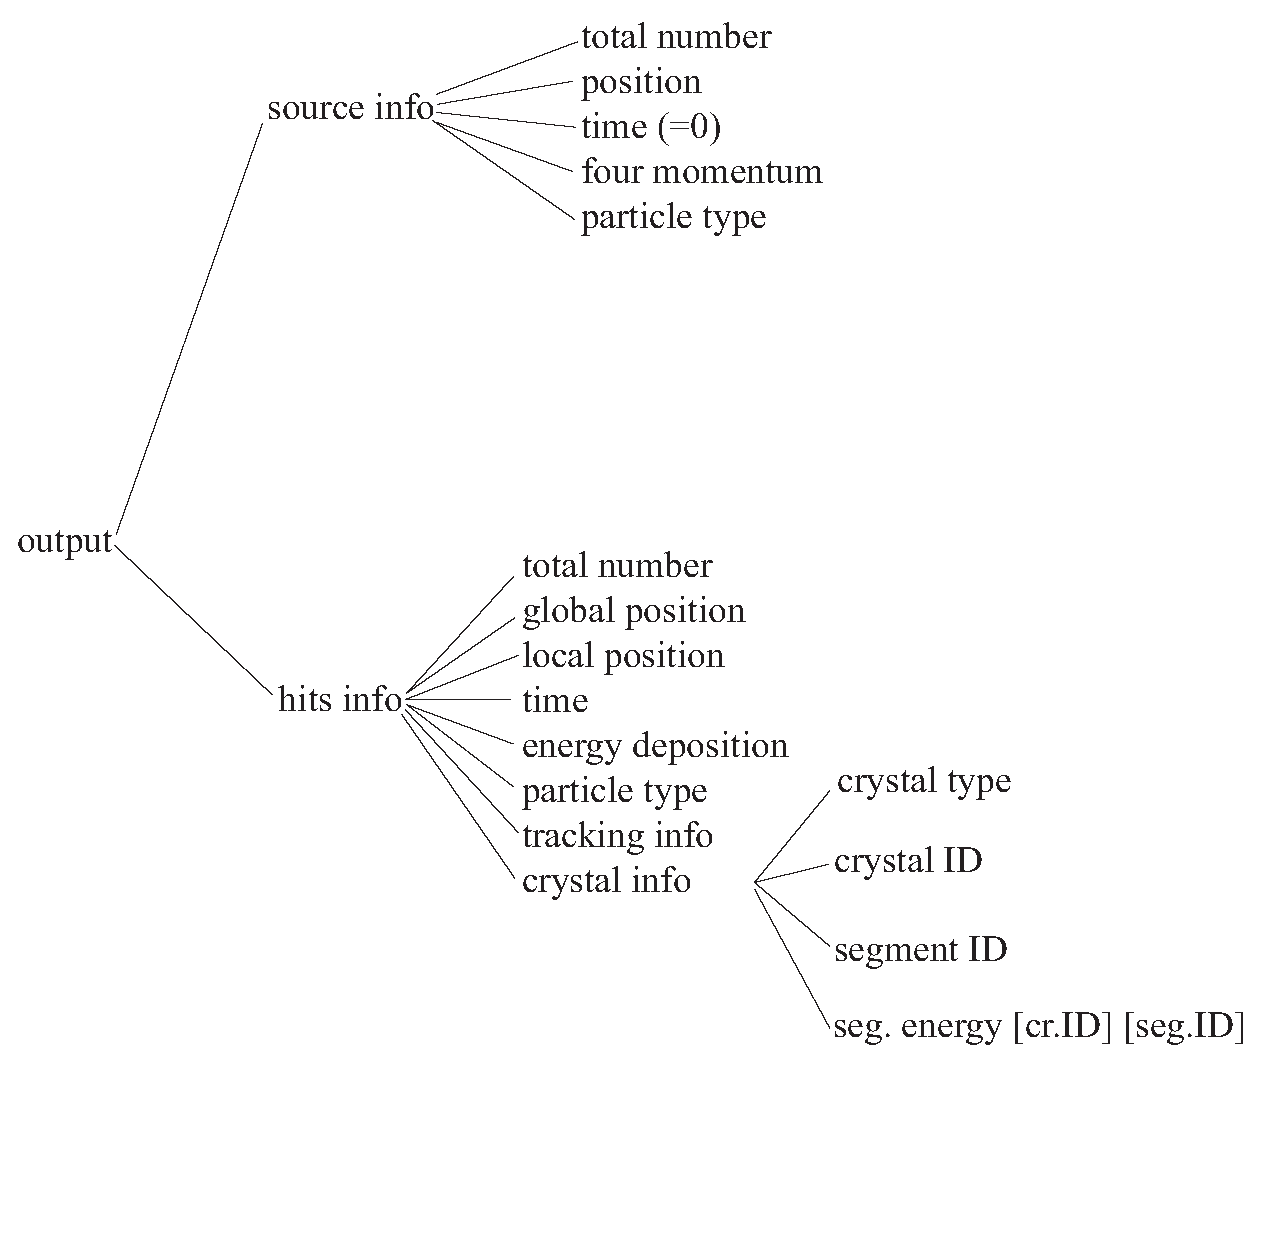
\includegraphics[scale=0.7]{figures/outputtree_big}
\caption{\small ROOT output tree of the class GEOutputCrystal. The segment energy is saved with respect to the crystal ID and the segment ID.}
\end{center}
\end{figure}

You can use the features of the class by typing:
\begin{lstlisting}
/MG/eventaction/rootscheme Crystal
/MG/eventaction/Crystal/save [source, hits, tracks, all]
\end{lstlisting}
\vspace{0.2cm}
The options in ``[  ]'' can be chosen from the ones listed above. You may use either one of them or a combination. In detail, they imply:\\
\begin{itemize}
 \item source - saves only the primary vertex and particles information
 \item hits - saves the hits and trajectories in the sensitive volumes
 \item tracks - saves all hits and all trajectories
 \item all - saves, well, all..
\end{itemize}
The default option is ``hits'', if the parameter is omitted.\\
\vspace{0.2cm}\\
Users can get the crystal type from the following ROOT branch:
\begin{lstlisting}
hitCrystalType[maxNhits]
\end{lstlisting}
The values correspond to the hit being in:
\begin{itemize}
\item -1 : not a sensitive volume at all
\item  0 : a sensitive volume but not a crystal
\item  1 : RolandI (unsegmented true coaxial p-type detector)
\item  2 : RolandII (6-fold segmented true coaxial p-type detector) 
\item  3 : RolandIII (18-fold segmented true coaxial p-type detector)  
\item  4 : Siegfried (18-fold segmented true coaxial n-type detector)
\end{itemize}
\vspace{0.2cm}
All the segments are arranged according to their local coordinate system. They are numbered from 1 for the first segment, R==0 and $\Phi$==0, counterclockwise and bottom up. The segmentation scheme and the segment numbering of the crystal ``Siegfried'' are shown in figure \ref{fig:segscheme}. Every event in a crystal is assigned to a detector segment according to the segmentation scheme using its z-, R- and $\Phi$- values.\\
\begin{figure}[h!]
 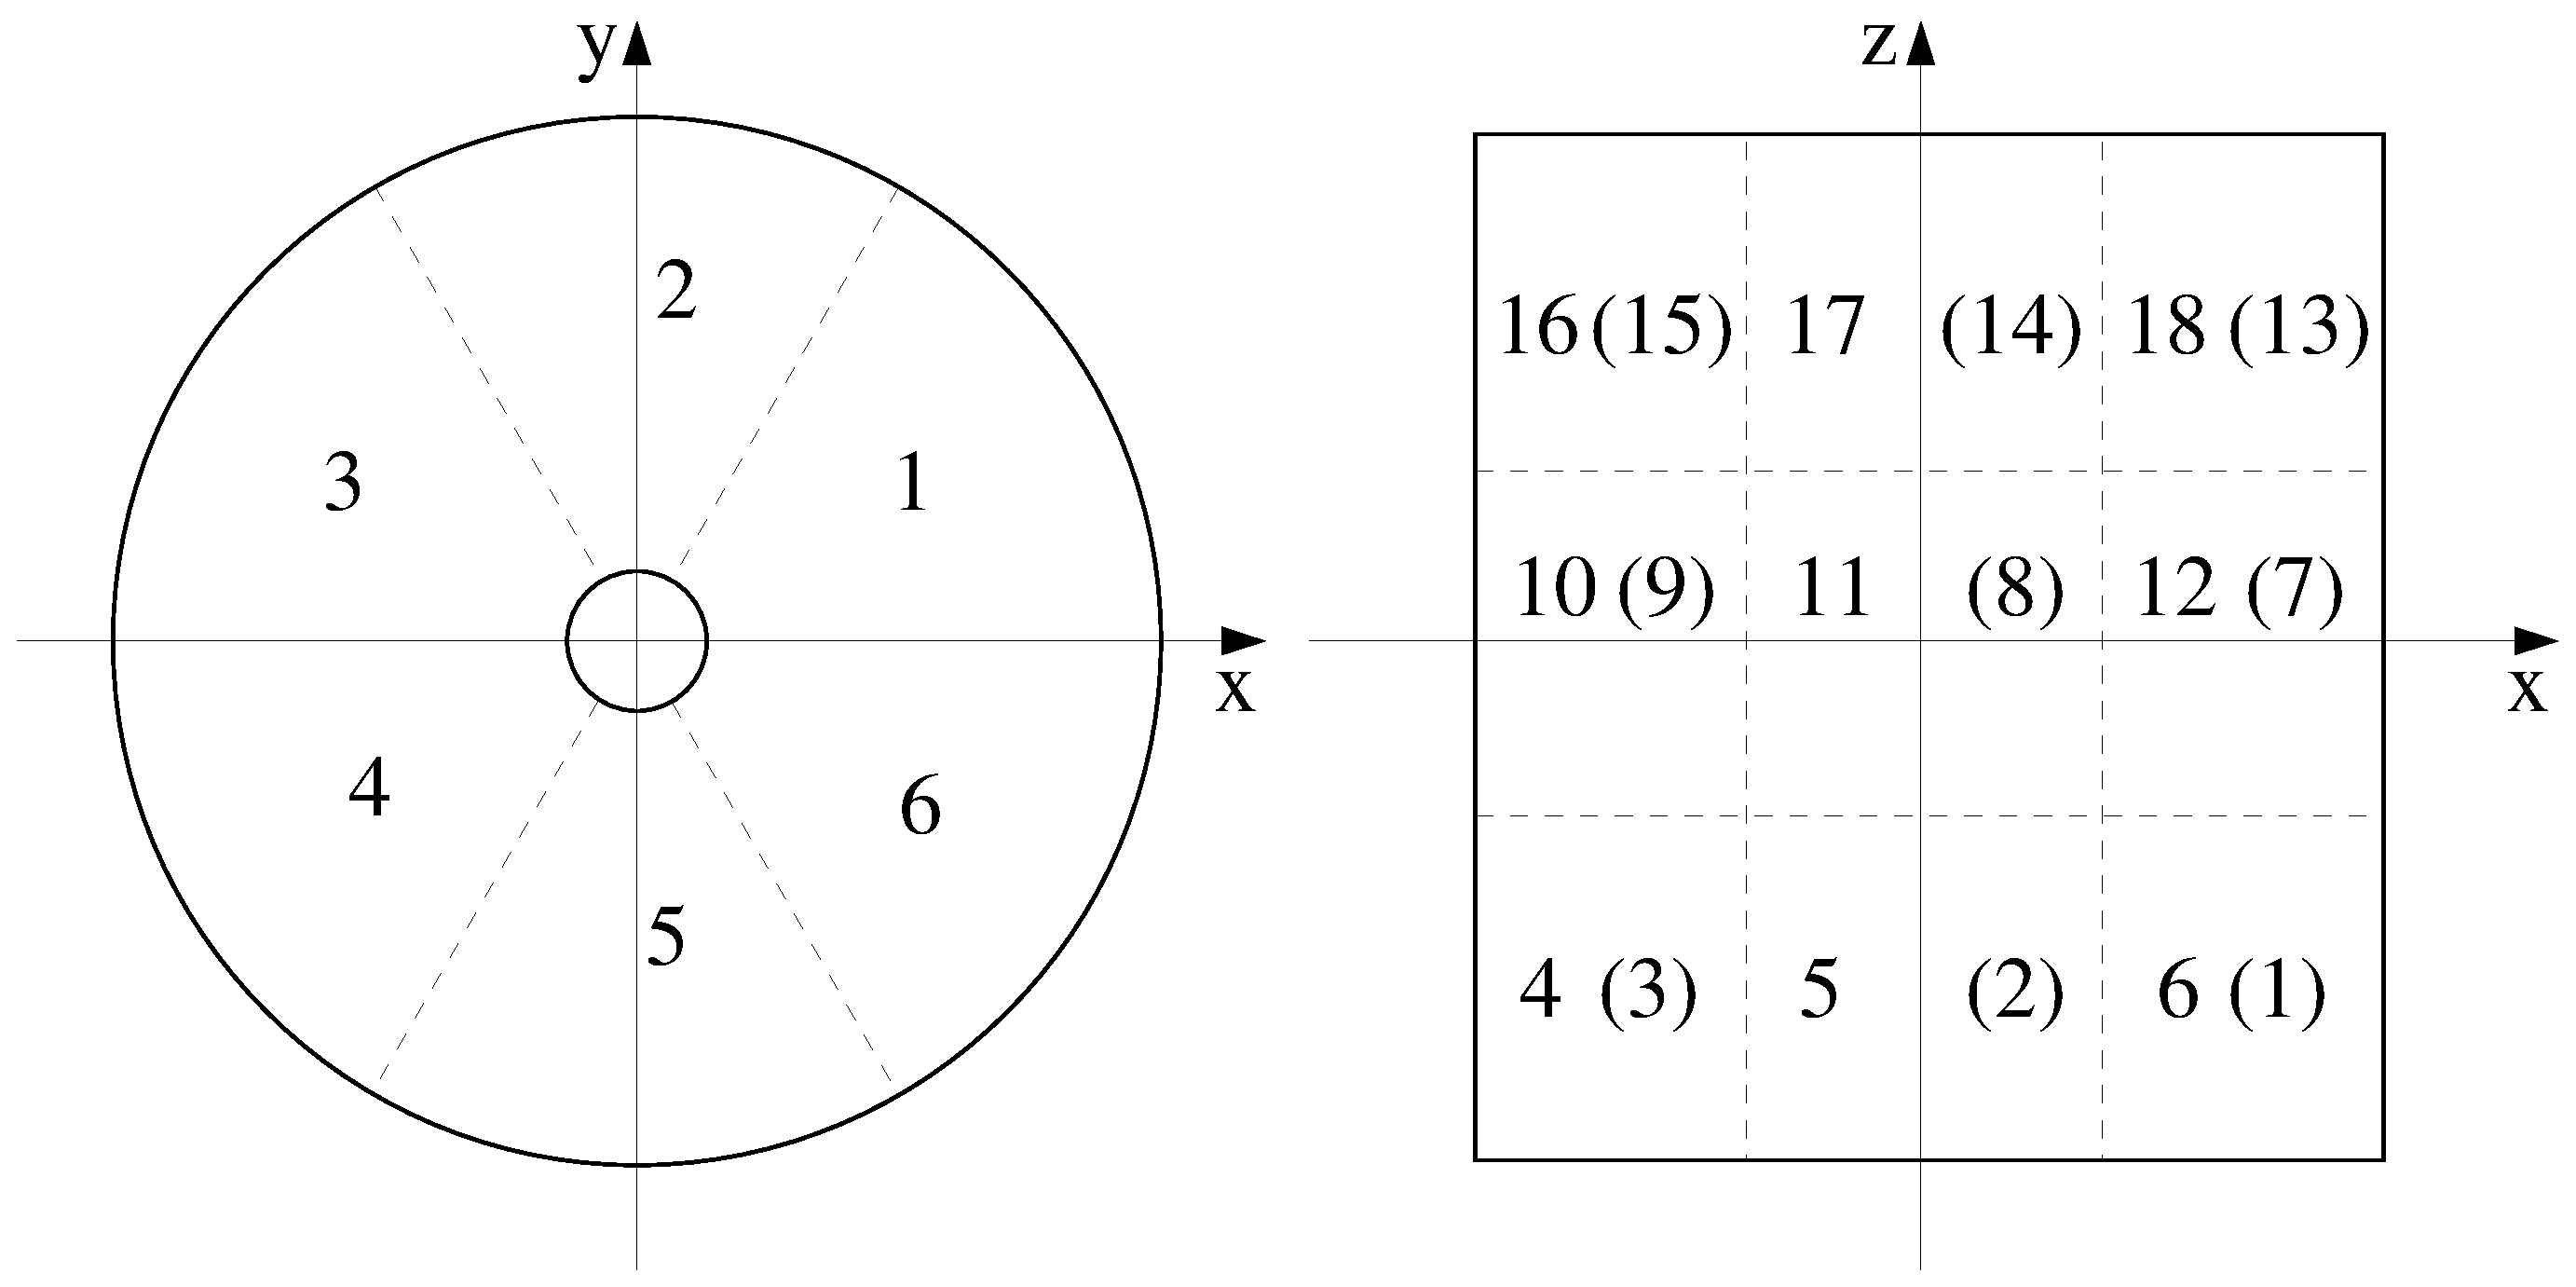
\includegraphics[scale=.3]{figures/segSchema}
\caption{Segmentation scheme for ``Siegfried''}
\end{figure} \label{fig:segscheme}
The segment shown in the ROOT branch is specified by the parameter:
\begin{lstlisting}
hitSegmentID[maxNhits]
\end{lstlisting}
The values correspond to:
\begin{itemize}
\item  -1 : not a sensitive volume at all
\item 0 : the whole volume which is sensitive (the whole detector)
\item 1 : the first segment  
\item 2 : the second segment
\item  ...
\end{itemize}
\vspace{0.2cm}
The crystal position in the \gerda \ array is given in the ROOT branch:
\begin{lstlisting}
hitCrystalID[maxNhits]
\end{lstlisting}
The values correspond to:
\begin{itemize}
\item -1 : not a sensitive volume at all
\item 0 : sensitive volume but not a crystal
\item 1 : the first crystal
\item 2 : the second crystal
\item  ...
\end{itemize}
The energy deposited in a segment of a crystal is saved in the ROOT branch:
\begin{lstlisting}
segmentEnergy[crystalID][segmentID]
\end{lstlisting}
Only positive crystal IDs can be used here, of course (negative values are not sensitive volumes). For crystal ID = 0, only segment ID = 0 is available (a volume with crystal ID = 0 is not a crystal). Crystal ID = n and segment ID = 0 shows you the energy deposited in the complete  n$^{th}$ crystal.\\
\subsubsection{Geometry developers' guide}
The implementation of segmentation and sensitive volumes is the pat that interests a developer. How this is done is explained here in a few steps.\\
The definition of a logical volume and a physical volume in \mage \ works as follows:\\
The geometry of a crystal is defined. It becomes a logical volume with attributes in the geometry construction class, e.g. in ``GEMunichTestStandDB'':
\begin{lstlisting}
fCrystalLogical 
= new G4LogicalVolume(CrystalTubs,	   //the name of the created geometry
		      enrichedGermanium,   //the material the crystal consists of
		     "CrystalLogical");	   //its name
\end{lstlisting}
This logical volume is inserted in the physical volume that is constructed like this:
\begin{lstlisting}
fCrystalPhysical
  = new G4PVPlacement(0, 			     //no rotation
		      G4ThreeVector(0,0,0),	     //translation position
		      fCrystalLogical,		     // pointer to its logical vol.
		      "CrystalPhysical",	     //its name
		      fCrystalMotherVolumeLogical,   //its mother logical volume
		      false,			     //no boolean operations
		      0);			     //its Copy Number
\end{lstlisting}
The physical volume name of a crystal defines its type. The class recognizes this and creates a segmentation scheme according to the
type. You don't have to define each segmentation in your geometry construction class.\\
You can take a simple G4Tubs object and name the physical volume ``siegfried''. The segmentation scheme predefined as ``siegfried''- scheme is implemented on the crystal. This means that hits inside this crystal have a segment ID according to their positions and the ``siegfried'' segmentation scheme.\\
A sensitive volume will be automatically recognized by the class from a physical volume.
You can change a usual physical volume to a sensitive one very easily: You only have to rename it as: ``PhysicalVolume'' $\longrightarrow$ ``sensitive\_PhysicalVolume''.\\
The hits in a sensitive volume are assigned to the segment of a detector using their local coordinates with the origin at the geometric center of the crystal:  x$_i$, y$_i$, z$_i$, T$_i$, p$_{x,i}$, p$_{y,i}$, p$_{z,i}$ and E$_{k,i}$ for the i$^{th}$ hit. The local coordinate system is also given in R$_i$, $\Phi$ $_i$ and z$_i$ with z$_i$==0 at half the height of the crystal.\\
The \gerda \ array consists of more than one detector. The position of each crystal is defined by its "CopyNo.".\\
Detectors in LAr are characterized by their logical volumes inside the mother volume "LAr" that are numbered top to bottom: 0, 1, 2... Hits inside these volumes will have a crystal ID (equals the CopyNo.+1): 1, 2, 3...\\
\vspace{0.2cm}\\
The definition of a physical volume in reality might look like this:
\begin{lstlisting}
fCrystalPhysical
  = new G4PVPlacement(0, 			     
		      G4ThreeVector(0,0,0),	     
		      fCrystalLogical,		     
		      "sensitive_siegfried",	     
		      fCrystalMotherVolumeLogical,   
		      false,			     
		      1);			     
\end{lstlisting}
The class GEOutputCrystal extracts the following information from this physical volume:\\
\begin{itemize}
\item It is a sensitive volume with the segmentation scheme of the crystal siegfried (the \textbf{crystal type }is defined).
\item The copy number of the crystal is 1, its \textbf{crystal ID} is 2 according to the scheme mentioned above.
\end{itemize}
If a hit is in segment 15 of ``Siegfried'', for example, this means:
\begin{itemize}
\item hitCrystalType = 4
\item hitCrystalID = 2
\item hitSegmentID = 15
\end{itemize}



\section{Majorana Output}
\label{IO_Majorana}
